% ============================================================
%  CLOSED-LOOP CONTROLLERS & PID CONTROL — STUDY GUIDE
%  For SCADA Automation Engineers
%  Covers 10 chapters: Intro through Simulation Lab
% ============================================================
\documentclass[12pt,twoside,openright]{memoir}

% ── Encoding & fonts ─────────────────────────────────────────
\usepackage[T1]{fontenc}
\usepackage[utf8]{inputenc}
\usepackage{lmodern}
\usepackage{microtype}
\usepackage{palatino}
\usepackage[scaled=0.85]{beramono}

% ── Page geometry ────────────────────────────────────────────
\usepackage[
  top=1.25in, bottom=1.25in,
  inner=1.5in, outer=1.0in,
  marginparwidth=0.8in, marginparsep=0.1in
]{geometry}

% ── Colors ───────────────────────────────────────────────────
\usepackage[dvipsnames,svgnames,x11names]{xcolor}
\definecolor{pidnavy}{HTML}{0D2137}
\definecolor{pidblue}{HTML}{1565C0}
\definecolor{pidcyan}{HTML}{0097A7}
\definecolor{pidorange}{HTML}{E65100}
\definecolor{pidgreen}{HTML}{2E7D32}
\definecolor{pidred}{HTML}{C62828}
\definecolor{pidyellow}{HTML}{F9A825}
\definecolor{rowlight}{HTML}{EFF6FF}
\definecolor{rowdark}{HTML}{DBEAFE}
\definecolor{codebg}{HTML}{F8F9FA}
\definecolor{frameborder}{HTML}{455A64}
\definecolor{covergray}{HTML}{ECEFF1}
\definecolor{warnbg}{HTML}{FFF3E0}
\definecolor{fieldbg}{HTML}{E8F5E9}

% ── Graphics & TikZ ──────────────────────────────────────────
\usepackage{graphicx}
\usepackage{tikz}
\usetikzlibrary{positioning,shapes.geometric,arrows.meta,decorations.pathreplacing,
                matrix,fit,backgrounds,calc,patterns,shadows.blur}
\usepackage{pgfplots}
\pgfplotsset{compat=1.18}

% ── Tables ───────────────────────────────────────────────────
\usepackage{booktabs}
\usepackage{tabularx}
\usepackage{array}
\usepackage{multirow}
\usepackage{colortbl}
\newcolumntype{L}[1]{>{\raggedright\arraybackslash}p{#1}}
\newcolumntype{C}[1]{>{\centering\arraybackslash}p{#1}}
\newcolumntype{R}[1]{>{\raggedleft\arraybackslash}p{#1}}

% ── Callout boxes (tcolorbox) ─────────────────────────────────
\usepackage[most,listings]{tcolorbox}

\newtcolorbox{keyconcept}[1][]{
  enhanced, breakable,
  colback=pidblue!8, colframe=pidblue, arc=4pt,
  fonttitle=\bfseries\sffamily\color{white}, title={Key Concept},
  attach boxed title to top left={yshift=-2mm, xshift=6mm},
  boxed title style={colback=pidblue, arc=3pt},
  #1
}

\newtcolorbox{warningbox}[1][]{
  enhanced, breakable,
  colback=warnbg, colframe=pidorange, arc=4pt,
  fonttitle=\bfseries\sffamily\color{white}, title={WARNING},
  attach boxed title to top left={yshift=-2mm, xshift=6mm},
  boxed title style={colback=pidorange, arc=3pt},
  #1
}

\newtcolorbox{example}[2][]{
  enhanced, breakable,
  colback=pidgreen!6, colframe=pidgreen, arc=4pt,
  fonttitle=\bfseries\sffamily\color{white}, title={Example: #2},
  attach boxed title to top left={yshift=-2mm, xshift=6mm},
  boxed title style={colback=pidgreen, arc=3pt},
  #1
}

\newtcolorbox{fieldnote}[1][]{
  enhanced, breakable,
  colback=fieldbg, colframe=pidgreen!60!black, arc=4pt,
  fonttitle=\bfseries\sffamily\color{white}, title={Field Note},
  attach boxed title to top left={yshift=-2mm, xshift=6mm},
  boxed title style={colback=pidgreen!70!black, arc=3pt},
  #1
}

\newtcolorbox{quickref}[1][]{
  enhanced, breakable,
  colback=pidyellow!15, colframe=pidyellow!80!black, arc=4pt,
  fonttitle=\bfseries\sffamily, title={Quick Reference},
  attach boxed title to top left={yshift=-2mm, xshift=6mm},
  boxed title style={colback=pidyellow!80!black, arc=3pt},
  #1
}

\newtcolorbox{commonmistakes}[1][]{
  enhanced, breakable,
  colback=pidred!5, colframe=pidred, arc=4pt,
  fonttitle=\bfseries\sffamily\color{white}, title={Common Mistakes},
  attach boxed title to top left={yshift=-2mm, xshift=6mm},
  boxed title style={colback=pidred, arc=3pt},
  #1
}

% ── Code listings ─────────────────────────────────────────────
\usepackage{listings}
\lstdefinestyle{codestyle}{
  basicstyle=\ttfamily\small,
  backgroundcolor=\color{codebg},
  frame=single, framerule=0.5pt, rulecolor=\color{frameborder},
  breaklines=true, keepspaces=true,
  xleftmargin=10pt, xrightmargin=10pt,
  aboveskip=6pt, belowskip=6pt,
  showstringspaces=false
}
\lstset{style=codestyle}

% ── Headers & footers ────────────────────────────────────────
\usepackage{fancyhdr}
\pagestyle{fancy}
\fancyhf{}
\fancyhead[LE]{\small\sffamily\color{pidblue}\leftmark}
\fancyhead[RO]{\small\sffamily\color{pidblue}\rightmark}
\fancyfoot[LE,RO]{\small\sffamily\thepage}
\fancyfoot[CO,CE]{\small\sffamily\color{gray}PID Control Study Guide}
\renewcommand{\headrulewidth}{0.4pt}
\renewcommand{\footrulewidth}{0.2pt}

% ── Hyperref ──────────────────────────────────────────────────
\usepackage[
  colorlinks=true,
  linkcolor=pidblue,
  urlcolor=pidcyan,
  citecolor=pidgreen,
  pdfauthor={Ricardo Barbosa},
  pdftitle={Closed-Loop Controllers \& PID Control --- Study Guide},
  pdfsubject={Process Control and PID Tuning},
  pdfkeywords={PID, closed-loop, SCADA, process control, tuning, FOPDT},
  bookmarks=true, bookmarksnumbered=true
]{hyperref}

% ── Misc ──────────────────────────────────────────────────────
\usepackage{enumitem}
\usepackage{amsmath}
\usepackage{amssymb}
\usepackage{soul}
\usepackage{mdframed}

% ── Memoir chapter style ──────────────────────────────────────
\makechapterstyle{pid}{%
  \renewcommand{\chapnamefont}{\normalfont\Large\sffamily\color{pidblue}}
  \renewcommand{\chapnumfont}{\normalfont\fontsize{56}{56}\bfseries\sffamily\color{pidblue!25}}
  \renewcommand{\chaptitlefont}{\normalfont\Huge\bfseries\sffamily\color{pidnavy}}
  \renewcommand{\printchapternum}{%
    \begin{tikzpicture}[remember picture]
      \node[fill=pidblue!10, rounded corners=6pt,
            inner sep=8pt, minimum width=3cm]{%
        \chapnumfont\thechapter};
    \end{tikzpicture}
  }
  \renewcommand{\afterchapternum}{\par\vspace{4pt}}
  \renewcommand{\afterchaptertitle}{%
    \par\vspace{4pt}
    
\begin{tikzpicture}
      \draw[pidblue, line width=2.5pt] (0,0) -- (\textwidth,0);
      \draw[pidorange, line width=1.2pt] (0,-3pt) -- (3cm,-3pt);
    \end{tikzpicture}
    \par\vspace{16pt}
  }
}
\chapterstyle{pid}

\setsecheadstyle{\large\bfseries\sffamily\color{pidblue}}
\setsubsecheadstyle{\normalsize\bfseries\sffamily\color{pidnavy}}
\setsubsubsecheadstyle{\normalsize\itshape\sffamily\color{pidnavy}}

% ── Helper macros ─────────────────────────────────────────────
\newcommand{\param}[1]{\texttt{#1}}

% =============================================================
%  DOCUMENT
% =============================================================
\begin{document}

% ── Cover page ────────────────────────────────────────────────
\begin{titlingpage}
\begin{tikzpicture}[remember picture, overlay]
  \fill[pidnavy] (current page.north west) rectangle
    ([yshift=-3.5in] current page.north east);
  \fill[pidblue!80] ([yshift=-3.5in] current page.north west)
    rectangle ([yshift=-3.7in] current page.north east);
  \fill[pidorange] ([yshift=-3.7in] current page.north west)
    rectangle ([yshift=-3.75in] current page.north east);
\end{tikzpicture}

\vspace*{0.5in}
{\color{white}\fontsize{11}{13}\sffamily\bfseries SCADA AUTOMATION ENGINEERING SERIES}
\vspace{0.15in}

{\color{pidcyan}\fontsize{40}{44}\bfseries\sffamily Closed-Loop Controllers}\\[6pt]
{\color{white}\fontsize{40}{44}\bfseries\sffamily \& PID Control}
\vspace{0.1in}

{\color{white!70}\fontsize{14}{18}\sffamily Study Guide for Process \& SCADA Engineers}

\vspace{1.9in}
\begin{flushleft}
{\large\sffamily\bfseries Ricardo Barbosa}\\[4pt]
{\sffamily\color{gray} NERC-Certified EDF Operator · MS AI Candidate, JHU}\\[2pt]
{\sffamily\color{gray} May 2026}
\end{flushleft}
\vfill
\end{titlingpage}

\frontmatter
\tableofcontents
\mainmatter

% =============================================================
\chapter{What Is Closed-Loop Control?}
% =============================================================

\section{Open-Loop vs.\ Closed-Loop}

Every industrial control system makes a fundamental design choice: does the controller measure what it's producing and adjust accordingly, or does it apply a fixed output and hope for the best?

\textbf{Open-loop control} applies a control action based solely on a predetermined input---no measurement of the actual output. A conveyor belt running at a fixed speed, a heating element at a fixed power level, a timer-controlled irrigation valve: none of these care what's happening in the process. They execute their programmed action regardless of the result.

\textbf{Closed-loop (feedback) control} measures the actual process output, compares it to the desired value, and continuously adjusts the manipulated variable to minimize the error. This feedback path is what closes the loop.

\begin{keyconcept}
Open-loop control is like driving with your eyes closed---technically possible, catastrophically wrong when anything changes. A closed-loop system measures where you actually are, computes the correction, and acts on it. Every cycle.
\end{keyconcept}

\section{The Feedback Loop Structure}

Every closed-loop control system---regardless of what variable is being controlled or what technology implements it---has the same fundamental structure:

\begin{center}
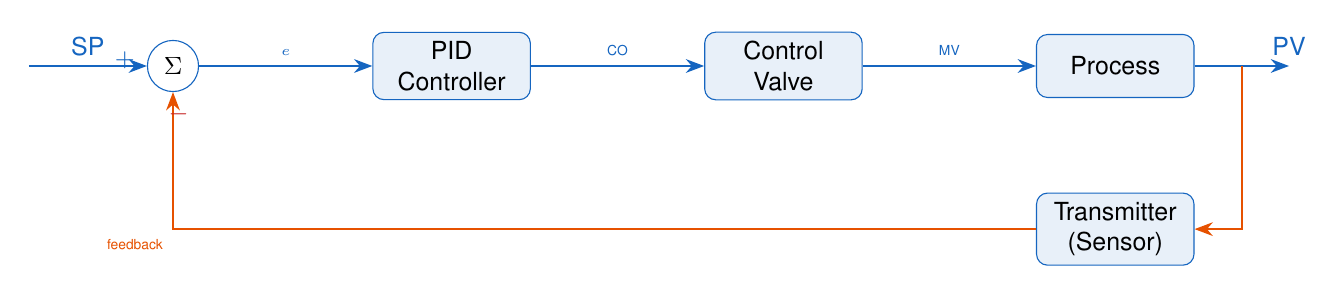
\begin{tikzpicture}[
  node distance=1.8cm and 2.2cm,
  block/.style={draw=pidblue, fill=pidblue!10, rounded corners=4pt,
                minimum width=2cm, minimum height=0.8cm,
                font=\small\sffamily, align=center},
  sum/.style={draw=pidblue, circle, minimum size=0.6cm, font=\small\bfseries},
  arrow/.style={-Stealth, thick, pidblue},
  feedback/.style={-Stealth, thick, pidorange}
]
  \node[sum] (sum) {$\Sigma$};
  \node[block, right=of sum] (ctrl) {PID\\Controller};
  \node[block, right=of ctrl] (valve) {Control\\Valve};
  \node[block, right=of valve] (proc) {Process};
  \node[block, below=1.2cm of proc] (sensor) {Transmitter\\(Sensor)};

  % SP input
  \draw[arrow] ([xshift=-1.5cm]sum.west) -- node[above,font=\small\sffamily]{SP} (sum.west);
  % Forward path
  \draw[arrow] (sum) -- node[above,font=\tiny\sffamily]{$e$} (ctrl);
  \draw[arrow] (ctrl) -- node[above,font=\tiny\sffamily]{CO} (valve);
  \draw[arrow] (valve) -- node[above,font=\tiny\sffamily]{MV} (proc);
  % PV output tap
  \draw[arrow] (proc.east) -- ++(1.2,0) node[above,font=\small\sffamily]{PV};
  % Feedback path
  \draw[feedback] (proc.east) ++(0.6,0) |- (sensor.east);
  \draw[feedback] (sensor.west) -| node[below left,font=\tiny\sffamily,pidorange]{feedback} (sum.south);
  % Negative sign
  \node[font=\small\bfseries, pidred] at ([xshift=2pt,yshift=-8pt]sum.south) {$-$};
  \node[font=\small\bfseries, pidblue] at ([xshift=-8pt,yshift=2pt]sum.west) {$+$};
\end{tikzpicture}
\end{center}

\begin{description}[leftmargin=2em, labelwidth=2em]
  \item[SP] Setpoint --- the desired value of the process variable.
  \item[$e$] Error = SP $-$ PV --- the deviation the controller must eliminate.
  \item[CO] Controller Output --- the signal sent to the final control element (typically 4--20\,mA or 0--100\%).
  \item[MV] Manipulated Variable --- the physical quantity changed by the actuator.
  \item[PV] Process Variable --- the measured output of the process.
\end{description}

\section{Industrial Examples}

\textbf{Tank Level Control.} A level transmitter measures liquid in a vessel (PV). The desired level is the setpoint (SP). The inlet control valve position is determined by the PID output. If a downstream pump increases its demand, the level drops, error increases, the controller opens the inlet valve---automatically, continuously, without operator intervention.

\textbf{Heat Exchanger Temperature.} Steam flow controls the outlet temperature of a process fluid. PV = outlet temperature. SP = desired temperature. CO drives the steam valve. A drop in steam header pressure is a disturbance; the controller detects the resulting temperature drop and opens the steam valve to compensate.

\textbf{Boiler Drum Pressure.} PV = drum pressure. SP = operating pressure. CO controls the fuel valve (firing rate). Steam demand changes are disturbances. The feedback loop maintains pressure within tight limits automatically.

% =============================================================
\chapter{Control Loop Fundamentals}
% =============================================================

\section{Setpoint, Process Variable, and Error}

The three most fundamental quantities in any control loop:

\begin{center}
\begin{tabular}{@{}L{2.5cm}L{3.5cm}L{8cm}@{}}
\toprule
\rowcolor{rowdark}
\textbf{Symbol} & \textbf{Name} & \textbf{Definition} \\
\midrule
SP & Setpoint & The target value an operator or system specifies. \\
\rowcolor{rowlight}
PV & Process Variable & The measured actual value of the controlled variable. \\
$e$ & Error & $e = \text{SP} - \text{PV}$. The deviation the controller acts to eliminate. \\
\rowcolor{rowlight}
CO & Controller Output & The signal sent to the final control element (0--100\%). \\
MV & Manipulated Variable & The physical quantity adjusted to control the PV. \\
\bottomrule
\end{tabular}
\end{center}

\section{Disturbances and Why Feedback Is Necessary}

A \textbf{disturbance} is any external influence that moves the PV away from SP without the controller doing anything. Without feedback, the controller has no way to detect or correct disturbances. With feedback, the loop automatically detects the error and corrects.

Common disturbances in process plants: ambient temperature changes, feed composition shifts, upstream pressure fluctuations, heat transfer surface fouling, and changes in load (downstream demand).

\section{Direct vs.\ Reverse Action}

Controller action determines the sign of the controller's response:

\begin{description}
  \item[Reverse Acting] When PV increases above SP, CO decreases. Standard for most control loops where a higher PV requires less input (e.g., temperature with a heater).
  \item[Direct Acting] When PV increases, CO increases. Used when a higher PV requires more of something (e.g., cooling water valve on a heat exchanger).
\end{description}

\begin{warningbox}
Wrong action setting = positive feedback. The loop will slam to a limit in seconds. This looks exactly like severely aggressive tuning. Check the action setting before adjusting tuning constants.
\end{warningbox}

% =============================================================
\chapter{P, I, and D --- What Each Does}
% =============================================================

\section{The PID Equation}

\begin{tcolorbox}[
  enhanced, breakable,
  colback=pidnavy!98, colframe=pidblue, arc=6pt,
  title={\sffamily\bfseries\color{white} The PID Control Law},
  fonttitle=\bfseries\sffamily,
  attach boxed title to top left={yshift=-2mm, xshift=6mm},
  boxed title style={colback=pidblue, arc=3pt}
]
\vspace{4pt}
\begin{equation}
\boxed{u(t) = K_p \cdot e(t) \;+\; K_i \int_0^t e(\tau)\,d\tau \;+\; K_d \frac{de(t)}{dt}}
\end{equation}
\vspace{2pt}
\begin{center}
\begin{tabular}{@{}lll@{}}
$K_p \cdot e(t)$ & --- & \textcolor{pidcyan}{Proportional}: responds to current error \\
$K_i \int e\,d\tau$ & --- & \textcolor{pidyellow}{Integral}: eliminates steady-state offset \\
$K_d \frac{de}{dt}$ & --- & \textcolor{pidorange}{Derivative}: damps oscillation, predicts future error \\
\end{tabular}
\end{center}
\vspace{2pt}
\end{tcolorbox}

\section{Proportional Action}

Proportional output = $K_p \times e(t)$. Larger error produces larger output. Zero error, zero proportional contribution. A P-only controller always has steady-state offset because the only way to produce a non-zero CO at steady state is to have a non-zero error.

\section{Integral Action}

Integral action accumulates error over time. As long as any error exists---no matter how small---the integral term keeps adjusting the CO until error = 0. This eliminates steady-state offset.

The danger: \textbf{integral windup}. When the output saturates (valve fully open/closed), the integral keeps accumulating. When saturation clears, the accumulated integral drives massive overshoot. Anti-windup mechanisms (clamping or back-calculation) prevent this.

\section{Derivative Action}

Derivative action responds to the \emph{rate of change} of error. If the PV is approaching SP rapidly, derivative reduces the CO before the target is reached---damping the response and reducing overshoot.

\begin{commonmistakes}
\textbf{Derivative kick:} If derivative is computed on error (not PV), a step change in SP produces an instantaneous infinite rate-of-change in error, causing a massive CO spike. Apply derivative to PV, not error, to prevent this. Verify which mode your PLC's PID block uses.
\end{commonmistakes}

% =============================================================
\chapter{Tuning Methods}
% =============================================================

\section{Open-Loop Step Test (Process Reaction Curve)}

Before applying any tuning formula, identify the process. Put the controller in manual, wait for steady state, step the CO by 5--10\%, and record the PV response. Extract:
\begin{itemize}
  \item $K$ = Process gain = $\Delta\text{PV} / \Delta\text{CO}$
  \item $\tau$ = Time constant = time for PV to reach 63.2\% of total change (after dead time)
  \item $\theta$ = Dead time = delay before PV starts responding
\end{itemize}
This yields the FOPDT model: $G(s) = K e^{-\theta s} / (\tau s + 1)$.

\section{Ziegler-Nichols Closed-Loop Method}

\begin{enumerate}
  \item Set Ki = 0, Kd = 0 (P-only).
  \item Increase Kp until sustained oscillation is achieved. This is the \textbf{ultimate gain} $K_u$.
  \item Measure the oscillation period $T_u$.
  \item Apply the table below.
\end{enumerate}

\begin{tcolorbox}[
  enhanced,
  colback=pidblue!6, colframe=pidblue, arc=4pt,
  title={\sffamily\bfseries\color{white} Ziegler-Nichols Tuning Table},
  attach boxed title to top left={yshift=-2mm, xshift=6mm},
  boxed title style={colback=pidblue, arc=3pt}
]
\begin{center}
\begin{tabular}{@{}L{3cm}C{3cm}C{3cm}C{3cm}@{}}
\toprule
\rowcolor{pidblue!15}
\textbf{Controller} & $K_p$ & $T_i$ & $T_d$ \\
\midrule
P only          & $0.50\, K_u$  & ---           & --- \\
\rowcolor{rowlight}
PI              & $0.45\, K_u$  & $T_u / 1.2$   & --- \\
PID             & $0.60\, K_u$  & $T_u / 2$     & $T_u / 8$ \\
\bottomrule
\end{tabular}
\end{center}
\end{tcolorbox}

\begin{warningbox}
Ziegler-Nichols produces aggressive (quarter-decay) tuning. Apply a detuning factor of 0.5--0.7 to Kp before commissioning. Use as a starting point only.
\end{warningbox}

\section{Lambda Tuning (IMC-Based)}

Lambda tuning requires step test data (K, $\tau$, $\theta$) and a desired closed-loop time constant $\lambda$:

\[
K_p = \frac{\tau}{K(\lambda + \theta)}, \qquad T_i = \tau
\]

Choose $\lambda \geq \theta$. Conservative: $\lambda = 2\theta$--$4\theta$. Lambda tuning is robust and directly relates to a physical performance specification.

% =============================================================
\chapter{Process Dynamics}
% =============================================================

\section{FOPDT Model}

The First-Order Plus Dead Time (FOPDT) model approximates most industrial processes:
\[
G(s) = \frac{K \, e^{-\theta s}}{\tau s + 1}
\]
The three parameters ($K$, $\tau$, $\theta$) fully characterize the process for tuning purposes.

\section{Self-Regulating vs.\ Integrating Processes}

\textbf{Self-regulating:} The PV naturally reaches a new steady state if the CO is held constant. Temperature, pressure, flow loops. Standard PID tuning applies.

\textbf{Integrating (non-self-regulating):} The PV ramps indefinitely if CO is held constant unless CO exactly matches the load. Tank level is the classic example. A P-only or PD controller is often preferred---adding integral to a level loop creates a double-integrator that destabilizes easily.

\section{Dead Time: The Enemy of Control}

Dead time ($\theta$) is the pure delay between a CO change and the first PV response. No tuning overcomes dead time. During $\theta$, the controller is blind. The only remedy is process design: shorter pipes, faster sensors, closer measurement points.

The $\tau/\theta$ ratio determines controllability. High $\tau/\theta$ (e.g., 10:1): easy. Low $\tau/\theta$ (e.g., 1:1): difficult---conservative tuning required.

% =============================================================
\chapter{Cascade \& Advanced Control}
% =============================================================

\section{Cascade Control}

Cascade control uses two loops in series. The primary (outer) loop controls the main process variable; its output becomes the setpoint for the secondary (inner) loop, which controls a faster intermediate variable.

\begin{keyconcept}
The inner loop must be 3--5$\times$ faster than the outer loop. Tune the inner loop first (outer in manual), then tune the outer loop with inner in auto.
\end{keyconcept}

Classic example: heat exchanger temperature (outer) cascaded to steam flow (inner). Steam supply pressure disturbances are rejected by the fast inner loop before they affect the slower outer temperature loop.

\section{Feedforward Control}

Feedforward measures a known disturbance and applies a compensating CO change \emph{before} the PV is affected. Requires a process model. Always paired with feedback to trim model errors.

\section{Ratio Control}

Maintains a fixed ratio between two process streams. The ``wild'' (uncontrolled) stream is measured; the ratio multiplied by it generates the setpoint for the ``controlled'' stream's flow controller.

% =============================================================
\chapter{Digital PID Implementation}
% =============================================================

\section{The Sampling Period}

A digital PID samples at interval $T$. Between samples, the controller is open-loop. Rules of thumb: $T \leq \tau/10$ and $T \leq \theta/4$. Typical values: flow 0.1--0.5\,s, temperature 1--10\,s, level 1--5\,s.

\section{Position vs.\ Velocity Algorithm}

\textbf{Position (absolute) form:}
\[
u[k] = K_p e[k] + K_i T \sum_{j=0}^{k} e[j] + K_d \frac{e[k]-e[k-1]}{T}
\]
Outputs absolute CO. Requires explicit anti-windup to prevent integral accumulation.

\textbf{Velocity (incremental) form:}
\[
\Delta u[k] = K_p\bigl(e[k]-e[k-1]\bigr) + K_i T \, e[k] + K_d \frac{e[k]-2e[k-1]+e[k-2]}{T}
\]
Outputs CO increment. Natural anti-windup. Bumpless transfer by initializing $\Delta u = 0$.

\section{Anti-Windup}

\textbf{Clamping:} Stop accumulating integral when output is saturated AND error is in the saturating direction.

\textbf{Back-calculation:} Apply a correction term proportional to $(u_\text{actual} - u_\text{desired})$ when saturated. Provides smoother exit from saturation.

% =============================================================
\chapter{PID in PLCs \& SCADA}
% =============================================================

\section{IEC 61131-3 CTRL\_PID Function Block}

Standard parameters include \param{ACTUAL} (PV input), \param{SET\_POINT} (SP), \param{KP}, \param{TI} (integral time in seconds), \param{TD} (derivative time), \param{MAN\_IN} (manual output value), \param{AUTO} (mode bool), and \param{OUT} (CO).

\section{Allen-Bradley (Rockwell) PID Instruction}

Key differences from IEC standard:
\begin{itemize}
  \item Uses independent parallel gains ($K_p$, $K_i$, $K_d$), not $T_i$/$T_d$ form
  \item $K_i$ is in \emph{repeats per minute}, not $1/T_i(\text{seconds})$: $K_i^\text{AB} = 1/T_i^\text{min}$
  \item PV scaled via MinEU/MaxEU parameters (engineering units)
  \item Derivative of PV vs.\ error is a configurable bit
\end{itemize}

\section{Bumpless Transfer}

Bumpless transfer prevents CO jumps when switching between manual and auto modes. On switch to auto: initialize the integral accumulator so the computed CO matches the current manual CO. On switch to manual: set the manual CO to the last auto CO value.

\section{PID Faceplate Elements}

A standard HMI PID faceplate exposes: SP entry (operator), PV display (read-only), CO bar (auto: display, manual: entry), mode toggle (Auto/Manual/Cascade), deviation alarm display, and output limits.

% =============================================================
\chapter{Troubleshooting Control Loops}
% =============================================================

\section{Diagnostic Approach}

Before changing any tuning constant, verify:
\begin{enumerate}
  \item PV transmitter calibrated and reading correctly
  \item Control valve stroking freely and linearly
  \item Loop in auto mode (not left in manual from previous shift)
  \item No mechanical issues: stiction, backlash, positioner failure
  \item Process has not changed: fouling, composition, load
\end{enumerate}

\begin{commonmistakes}
80\% of loop problems are \emph{not} tuning problems. Adjusting $K_p$ to compensate for a stuck valve treats the symptom. The valve sticks again next week.
\end{commonmistakes}

\section{Symptom Reference Table}

\begin{center}
\begin{tabular}{@{}L{3.5cm}L{4.5cm}L{5cm}@{}}
\toprule
\rowcolor{rowdark}
\textbf{Symptom} & \textbf{Likely Cause} & \textbf{Fix} \\
\midrule
Regular oscillation & $K_p$ too high or $T_i$ too fast & Reduce $K_p$ 30--50\%; increase $T_i$ \\
\rowcolor{rowlight}
Steady-state offset & Integral disabled or too slow & Enable/decrease $T_i$ \\
Sluggish response & $K_p$ too low or valve binding & Increase $K_p$; check valve \\
\rowcolor{rowlight}
Sawtooth PV, CO ramps then jumps & Valve stiction (limit cycling) & Service valve; positioner \\
Massive overshoot at startup & Integral windup & Enable anti-windup; configure SP ramp \\
\rowcolor{rowlight}
CO moves, PV does not follow & Valve/actuator mechanical failure & Inspect valve, positioner \\
\bottomrule
\end{tabular}
\end{center}

% =============================================================
\chapter{Simulation Lab}
% =============================================================

\section{Free Simulation Tools}

\begin{itemize}
  \item \textbf{MATLAB/Simulink} (student \$35/yr) --- industry standard, Control System Toolbox
  \item \textbf{Python \texttt{control} library} (\texttt{pip install control}) --- free, flexible
  \item \textbf{CADSIM Plus} --- free tier, process-oriented simulator
  \item \textbf{Excel spreadsheet} --- build it yourself; most instructive option
\end{itemize}

\section{Exercises}

\textbf{Exercise 1 --- Excel FOPDT Simulator.}
Implement discrete-time PID ($T = 0.5$\,s) controlling a FOPDT process ($K=1.5$, $\tau=30$\,s, $\theta=5$\,s). Plot SP, PV, CO. Tune by doubling $K_p$ until oscillation appears, then back off. Add integral. Observe windup if anti-windup is disabled.

\textbf{Exercise 2 --- Lambda Tuning Validation.}
Using the same process, calculate Lambda tuning constants with $\lambda = 2\theta = 10$\,s. Simulate. Compare rise time, overshoot, and settling time against Z-N open-loop tuning.

\textbf{Exercise 3 --- Valve Stiction Simulation.}
Add a deadband of $\pm 2\%$ to the valve model (valve does not move unless CO changes by more than 2\%). Observe limit cycling behavior. Compare the PV trend shape to the oscillation patterns in Chapter 9.

\textbf{Exercise 4 --- Process Type Comparison.}
Tune a self-regulating loop (temperature) and an integrating loop (level) with the same PID constants. Observe the dramatically different responses. Tune each appropriately and document the difference in required Kp, Ti.

\begin{fieldnote}
The simulation loop \emph{is} the study loop. Build it, break it deliberately, diagnose why it broke, fix it. A student who has caused and fixed integral windup, oscillation, offset, and valve stiction in simulation will outperform a student who only read about these phenomena every time, in the field, on day one.
\end{fieldnote}

\backmatter

% ── Quick reference appendix ──────────────────────────────────
\appendix
\chapter{Quick Reference}

\section{Tuning Rule Summary}

\begin{center}
\begin{tabular}{@{}L{3cm}C{2.5cm}C{2.5cm}C{2.5cm}C{3cm}@{}}
\toprule
\rowcolor{rowdark}
\textbf{Method} & $K_p$ & $T_i$ & $T_d$ & \textbf{Notes} \\
\midrule
Z-N (closed-loop) & $0.60\,K_u$ & $T_u/2$ & $T_u/8$ & Aggressive; detune \\
\rowcolor{rowlight}
Lambda PI & $\tau/[K(\lambda+\theta)]$ & $\tau$ & --- & Choose $\lambda \geq \theta$ \\
Cohen-Coon PI & See ch.\ 4 formulas & See ch.\ 4 & --- & Good for $\theta/\tau > 0.1$ \\
\bottomrule
\end{tabular}
\end{center}

\section{Rule-of-Thumb Starting Points}

\begin{center}
\begin{tabular}{@{}L{3cm}C{2.5cm}C{2.5cm}L{5cm}@{}}
\toprule
\rowcolor{rowdark}
\textbf{Loop Type} & $K_p$ & $T_i$ (min) & \textbf{Notes} \\
\midrule
Flow & 0.3--0.5 & 0.05--0.2 & Noisy; avoid derivative \\
\rowcolor{rowlight}
Liquid Level & 1--3 & 5--30 & Often P-only \\
Temperature & 1--5 & 2--10 & D sometimes helpful \\
\rowcolor{rowlight}
Gas Pressure & 2--5 & 0.5--3 & Can be fast \\
\bottomrule
\end{tabular}
\end{center}

\section{Professional Certification Prep}

\subsection{ISA CCST --- Certified Control Systems Technician}

Three levels based on experience (Level I: 5 years, Level II: 7 years, Level III: 13 years). Cost: approximately \$415 USD. Recertification required every 3 years.

\noindent Exam domains relevant to this guide:
\begin{itemize}
\item \textbf{Basic Continuous Control} --- PID control theory, DCS architecture, loop tuning, controller modes (P, PI, PID), control loop diagrams. This guide's Chapters 1--5 directly prepare for this domain.
\item \textbf{Advanced Control} --- Cascade control, feedforward, ratio control, split-range, override/select. Covered in this guide's Chapter 8.
\item \textbf{Integration and Software} --- Communication protocols (Modbus, HART, Fieldbus), SCADA integration, historian. Understanding PID in the context of SCADA tags is tested.
\item \textbf{Deployment and Maintenance} --- Startup procedures, troubleshooting oscillating loops, calibration, bump testing. Chapter 5 (tuning) and Chapter 9 (troubleshooting) apply.
\end{itemize}

\medskip
\noindent\textbf{Official Resources:} isa.org/certification/ccst, ISA CCST Body of Knowledge at isa.org/certification/ccst/ccst-body-of-knowledge

\subsection{ISA CAP --- Certified Automation Professional}

Target audience: automation engineers (mid-to-senior). Requirements: Bachelor's degree + 5 years experience (or equivalent). Cost: approximately \$500--\$750 USD. Format: 175 multiple-choice questions, 4-hour time limit. Recertification every 3 years.

\noindent Exam domains covered by this guide:
\begin{itemize}
\item \textbf{Basic Continuous Control (Domain 1)} --- PID fundamentals, control loop performance analysis, DCS systems. This guide provides thorough preparation.
\item \textbf{Advanced Control (Domain 3)} --- Model predictive control (MPC) concepts, cascade, feedforward, FOPDT model identification (28.3\%/63.2\% method). Chapters 6--8 of this guide are specifically CAP-aligned.
\item \textbf{Discrete, Sequencing, and Manufacturing Control (Domain 2)} --- Covered partially; PLC integration with PID loops.
\item \textbf{Project Work Structure (Domain 7)} --- Automation project lifecycle; PID loop tuning as a commissioning deliverable.
\end{itemize}

\medskip
\noindent\textbf{Official Resources:} isa.org/certification/cap, 2024 CAP Content Outline at isa.org/certification/cap/cap-body-of-knowledge

\end{document}
